\documentclass[a4paper]{article}
\usepackage[margin=1in]{geometry}
\usepackage[spanish]{babel}
\selectlanguage{spanish}
\usepackage[utf8]{inputenc}

\usepackage{hyperref}
\usepackage{graphicx}
\usepackage{float}

\setlength{\parindent}{2cm}
\setlength{\parskip}{4mm}

% colors for hyperlinks
% colored borders (false) colored text (true)
\hypersetup{colorlinks=true,citecolor=black,filecolor=black,linkcolor=black,urlcolor=black}

% package for bibliography
\usepackage[authoryear,round]{natbib}
% package for header
\usepackage[automark,headsepline]{scrlayer-scrpage}
\pagestyle{scrheadings}
\ihead[]{Emmanuel Arias}
% \ohead[]{\today}
\cfoot[]{\pagemark} 

\begin{document}
	\title{\vspace{5cm}
	\Huge Git: Configuración y primeros comandos
	}
	
	\vspace{5cm}

	\author{\Large \href{mailto:emmanuelarias@gmail.com}{Emmanuel Arias}}	
	
	\vspace{5cm}

	\date{}

	\maketitle
	
	\newpage
	% \tableofcontents
	%\newpage
	
\section{Configuración} % (fold)
\label{sec:configuracion}
Lo primero que necesitamos realizar una vez descargado e instalado
Git es su configuración.

Podemos configurar variables en tres ambientes, sistema, global y local.
Las variables se guardan en archivos.

\begin{itemize}
	\item Cuando configuramos una variable en el ambiente sistema, esta queda
	disponible para todo el sistema.  En sistemas Linux se guardan en 
	\verb|/etc/gitconfig| en sistemas Windows se guarda en
	\verb|C:\ProgramData\Git\config|.
	\item Cuando se configura en el ambiente global, esto significa que está
	disponible para un usuario en específico. Es decir que esa configuración
	va a estar disponible para todos los proyectos del usuario. Estos datos
	se guardan en el archivo \verb|~/.gitconfig| o \verb|C:\Users\\.gitignore|
	\item Cuando configuramos utilizando el ambiente local, estas variables solo
	se encuentran disponible para un proyecto dónde fue configurado.
\end{itemize}

Para configurar utilizamos el comando ``config", seguido por el argumento que
indique en qué ambiente queremos guardar esa información.

Normalmente, configuramos Git utilizando el ambiente global, ya que de esta
manera nos permitirá tener siempre disponible esta información para todos 
los proyectos que manejemos, en casos muy puntuales necesitaremos cambiar nuestra
información en algún proyecto, por lo que usaremos en ese caso la configuración 
``local"".

Primero, el comando tiene la siguiente forma:

\begin{verbatim}
	git config --system nombre.variable "valor"
	git config --global nombre.variable "valor"
	git config --local nombre.variable "valor"
\end{verbatim}

Como primer paso configuremos nuestro git con la información mínima
que necesitamos para darle autoría a nuestros trabajos.

\begin{verbatim}
	git config --global user.name "Emmanuel Arias"
	git config --global user.email "eamanu@yaerobi.com"
\end{verbatim}

Luego deberemos configurar un editor de texto que se abra cada vez que 
necesitemos hacer un ``commit". Para ello, necesitamos configurar la variable
core.editor seguido por el nombre del editor (esto funciona en Linux), o
el path al ejecutable en Windows. Por ejemplo, yo configuro para que mi editor
por defecto sea vim.

\begin{verbatim}
	git config --global core.editor "vim"
\end{verbatim}

\subsection{Configuración ssh}
\label{sec:sshconfig}

Cuando usamos Github cada vez que sincronizamos con nuestro repositorio local, 
esto es, cada vez que envíamos cambios a Github o queremos traer información
de Github (por ejemplo, clonar un repositorio, hacer un pull, que ya veremos
que es eso) Necesitamos autenticarnos. Para autenticarnos, la forma más sencilla
es escribiendo nuestro usuario y contraseña y eso es todo, pero para ellos
siempre tendremos que trabajar con el protocolo \textit{HTTP}. La otra forma
es utiliza \textit{ssh} y de esa manera nos evitamos escribir a cada rato
usario y contraseña, y bueno obviamente es más seguro.

Para ello, simplemente seguimos la documentación de Github y listo :)

\href{https://docs.github.com/es/github/authenticating-to-github/adding-a-new-ssh-key-to-your-github-account}{En este link podrá configurar Github con ssh en Windows, MacOS o Linux}

\section{Nuestro primer proyecto}

Para crear nuestro primer proyecto vamos a utilizar el comando ``init".
Ya depende de cada uno y su forma de trabajar, pero yo recomiendo ser organizado
y tener un directorio para guardar nuestros proyectos.

Entonces, vamos a crear nuestro primer proyecto. Primero debemos una carpeta con
el nombre del proyecto, y vamos a acceder a él. Lo pueden hacer desde la GUI, o 
por comandos, yo lo haré por comandos pero es lo mismo.

\begin{verbatim}
	mkdir MiPrimerProyectoGit
	cd MiPrimerProyectoGit
\end{verbatim}

\begin{figure}[H]
	\centering
	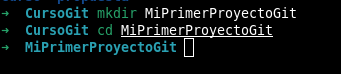
\includegraphics[width=0.7\linewidth]{img/miprimerproyecto}
	\label{fig:miprimerproyecto}
\end{figure}

(Eso equivale a botón derecho, Nueva Carpeta. Luego F2 y escribir el nombre
de la carpeta y por último presionar dos veces en la carpeta.)

Luego abriremos nuestra línea de comandos o Git Bash si estamos en Windows, y
escribiremos

\begin{verbatim}
	git init
\end{verbatim}

\begin{figure}[H]
	\centering
	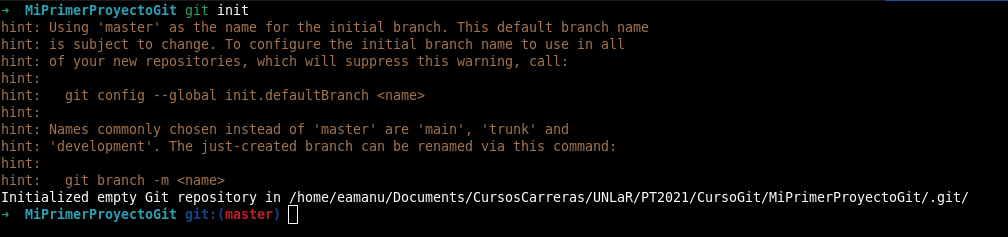
\includegraphics[width=0.7\linewidth]{img/miprimerproyecto2}
	\label{fig:miprimerproyecto2}
\end{figure}

Y listo! con esto ya tendremos nuestro proyecto creado. Ahora ya podemos empezar
a trabajar.

Podremos verificar que está creado si usamos el comando

\begin{verbatim}
	git status
\end{verbatim}

\begin{figure}[H]
	\centering
	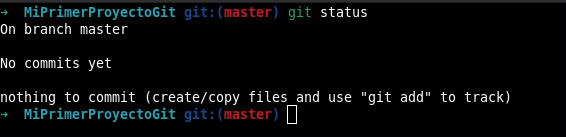
\includegraphics[width=0.7\linewidth]{img/miprimerproyecto3}
	\label{fig:miprimerproyecto3}
\end{figure}

\subsection{Agregando archivos al proyecto}

Por lo pronto vamos a hacer algo muy simple, vamos a crear un archivo
y vamos a escribir lo que sea, solo es un primer proyecto, ya tendremos
tiempo para cosas más avanzadas.

Creamos un archivo como lo harían normalmente, ojo, mejor si es texto plano,
para evitar algunas cuestiones que no vienen al caso por ahora.

En mi caso, solo pondré en ese archivo ``Este es mi primer proyecto", y el nombre?
cualquiera, puede ser... README.txt.

\begin{figure}[H]
	\centering
	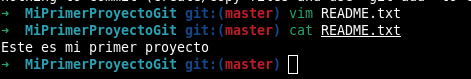
\includegraphics[width=0.7\linewidth]{img/miprimerproyecto4}
	\label{fig:miprimerproyecto4}
\end{figure}

Ahora hacemos un \verb|git status| para ver cómo avanzamos:

Bueno aparece en rojo nuestro archivo ``README.txt". Eso es bueno

Puntos a tener en cuenta hasta ahora:

\begin{itemize}
	\item Todos los comandos que estamos viendo, init, status, etc y los que
	veremos en breve, ya tendremos más tiempo de estudiarlos en otras
	unidades, primero hagamos funcionar Git, y luego veamos los detalles.
	\item Cuando hicieron el último \verb|git status| vieron más archivo o
	carpetas que README.txt: \textit{Houston, we've a problem}. Acá hay algo mal, y
	deberán volver al inicio.
\end{itemize}

Se acuerdan de la clase de las etapas o ``stages" de Git? Bueno, ahora README.txt
está en Untracked, no está en Git todavía. Vamos a agregarlo, para ello ejecutamos

\begin{verbatim}
	git add README.txt
\end{verbatim}

Ahora si hacemos git status aparecerá en otro color:

\begin{figure}[H]
	\centering
	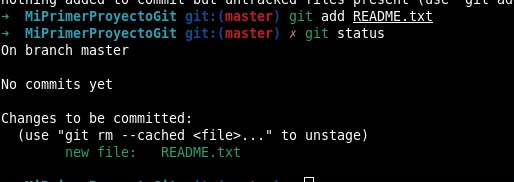
\includegraphics[width=0.7\linewidth]{img/miprimerproyecto5}
	\label{fig:miprimerproyecto5}
\end{figure}

Ahora está en Stagging. Vamos a agregarlo en el repositorio para que ya quede
guardada en la historia de Git.

Para ello hacemos 

\begin{verbatim}
	git commit
\end{verbatim}

Esto nos abrirá el editor que habíamos configurado en \ref{sec:configuracion} y 
escribimos un mensaje. Una vez escrito el mensaje, lo guardan y salen del editor.
En mi caso lo hago en vim (si por esas casualidades, utilizaron vim y no saben
salir del editor, aprieten el botón ESC y luego escriban \verb|:wq| y presionen
Enter, y listo.), y se ve así:

\begin{figure}[H]
	\centering
	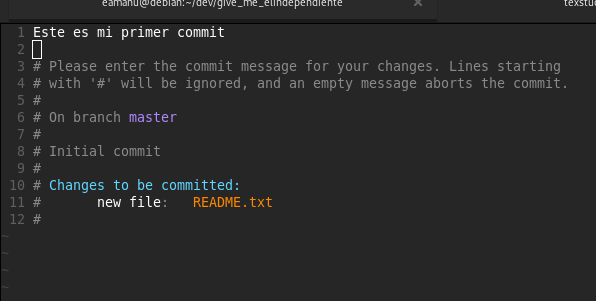
\includegraphics[width=0.7\linewidth]{img/miprimerproyecto6}
	\label{fig:miprimerproyecto6}
\end{figure}

Si ejecutan status verán que ya no hay nada nuevo, así que \textit{voilà},
tenemos nuestro primer commit realizado!!!.

¿Cómo lo vemos? Pueden ejecutar \verb|git show| o \verb|git log|.

\begin{figure}[H]
	\centering
	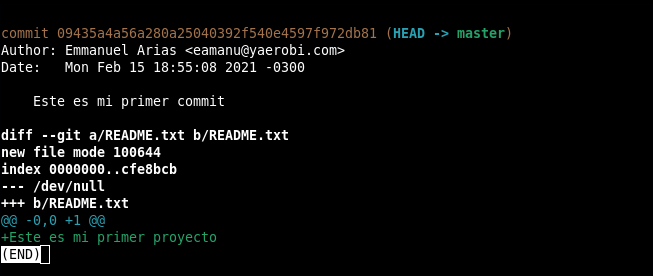
\includegraphics[width=0.7\linewidth]{img/miprimerproyecto7}
	\label{fig:miprimerproyecto7}
\end{figure}


\section{Vamos a Github}

Vamos a ingresar a Github, y creamos un nuevo repositorio, haciendo clic
en el botón que aparece a la izquierda que dice ``Nuevo":

\begin{figure}[H]
	\centering
	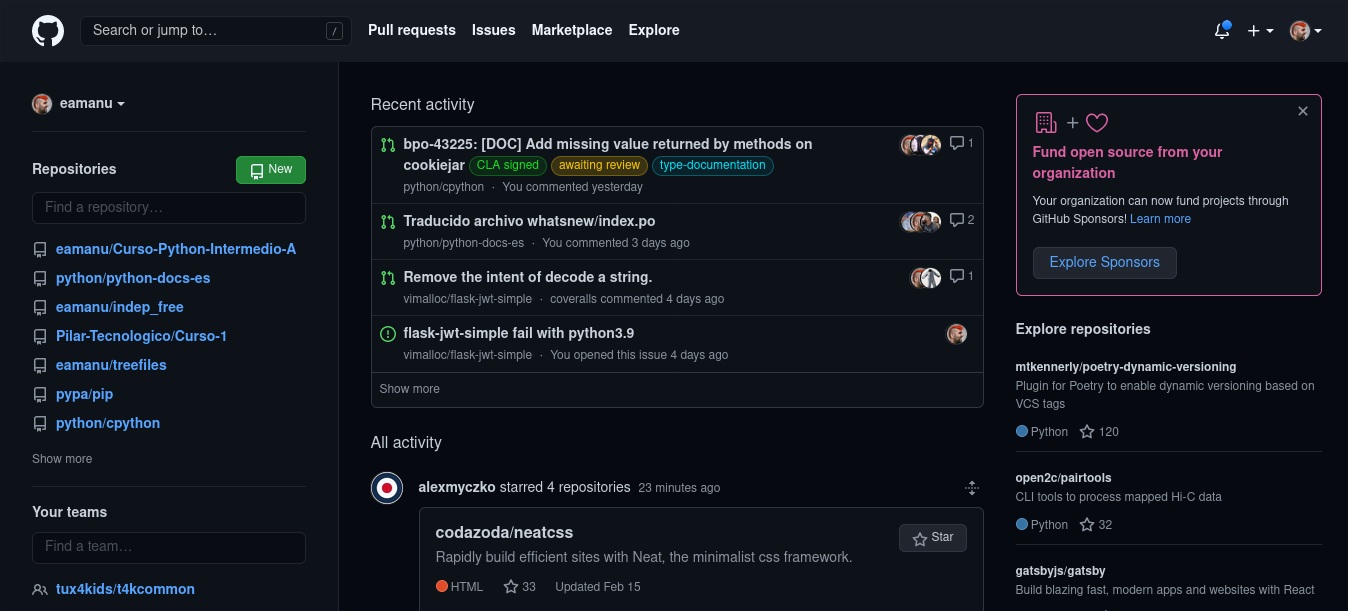
\includegraphics[width=0.7\linewidth]{img/miprimerproyecto8}
	\label{fig:miprimerproyecto8}
\end{figure}

Luego le ponemos un nombre al proyecto, mantengamos el mismo. Hacemos
clic en ``Public". Y en la última sección que nos pregunta si queremos
``inicializar el proyecto con" \textbf{NO seleccionamos ninguno}.

\begin{figure}[H]
	\centering
	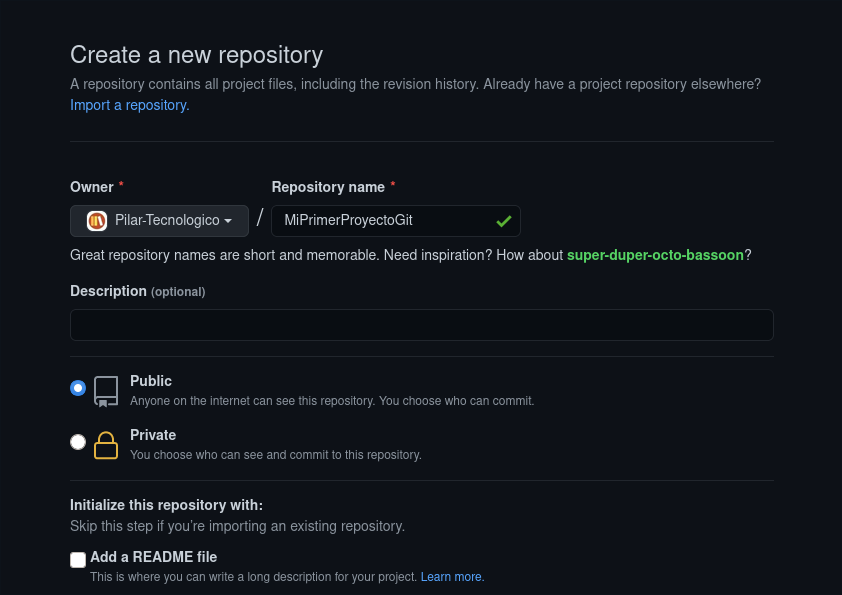
\includegraphics[width=0.7\linewidth]{img/miprimerproyecto9}
	\label{fig:miprimerproyecto9}
\end{figure}

Apretamos en el botón crear repositorio. Vamos a tener algo similar a esto:

\begin{figure}[H]
	\centering
	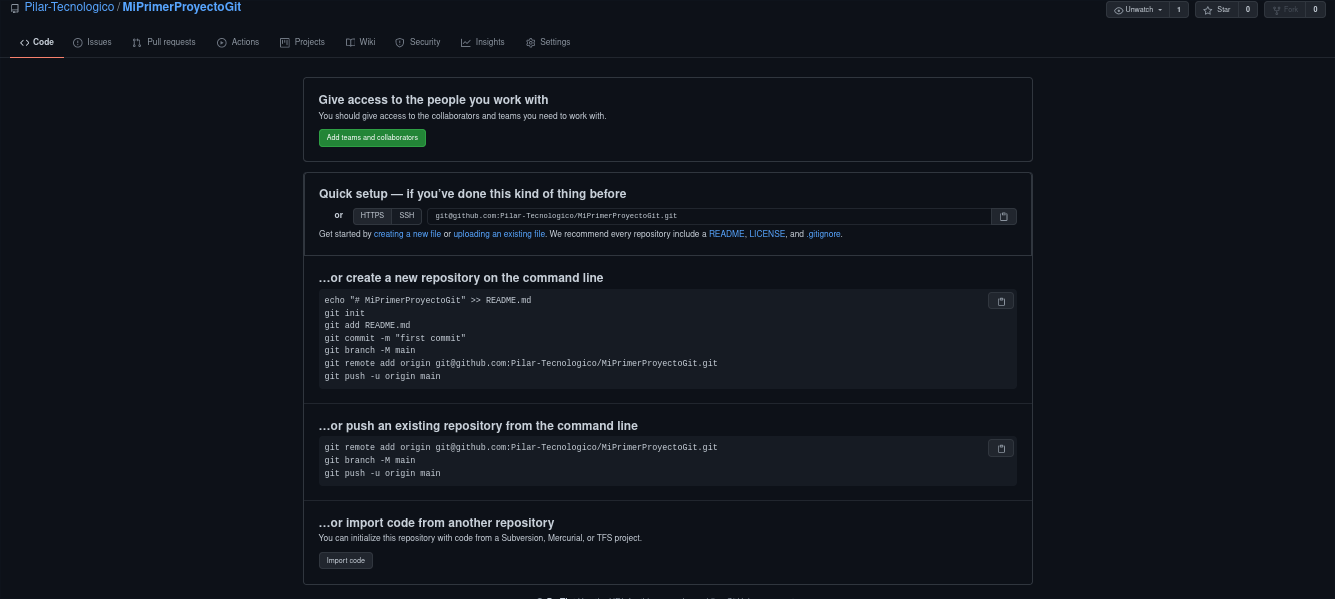
\includegraphics[width=0.7\linewidth]{img/miprimerproyecto10}
	\label{fig:miprimerproyecto10}
\end{figure}

Veremos que ya nos da mucha información de lo que debemos hacer a continuación
lo cual es bueno, nosotros ya creamos un proyecto, así que tenemos que hacer
lo que nos dice la sección ``push un proyecto existente desde la línea de comandos".

Antes que nada, si ya hemos configurado nuestro Github para que funcione con ssh
(\ref{sec:sshconfig}) elegimos la opción ssh que aparece arriba en la página, si
no lo hicimos, tendremos que seleccionar la opción http.

Simplemente copiamos línea a línea y eso es todo.

\begin{figure}[H]
	\centering
	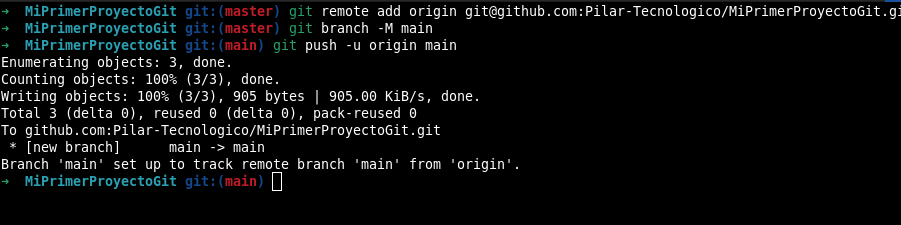
\includegraphics[width=0.7\linewidth]{img/miprimerproyecto11}
	\label{fig:miprimerproyecto11}
\end{figure}

Ahora si refrescamos la página, veremos que nuestro código ya está en Github.

\begin{figure}[H]
	\centering
	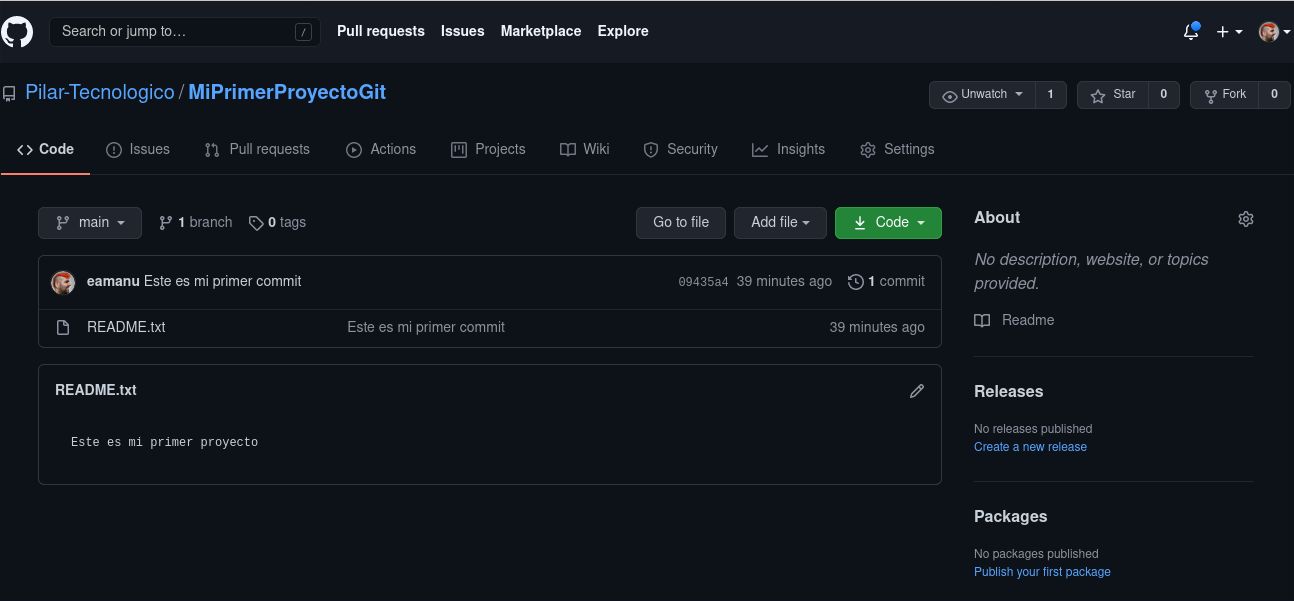
\includegraphics[width=0.7\linewidth]{img/miprimerproyecto12}
	\label{fig:miprimerproyecto12}
\end{figure}


\end{document}